% run "tikz2png filepath.tex" in terminal to create the png (see function at end of doc) using poppler
\documentclass{standalone}
\usepackage{tikz}
\tikzset{>=latex} % for LaTeX arrow head
\usetikzlibrary{tikzmark} % for subnode
%\usepackage{pgfpages}
%\pgfpagesuselayout{resize to}[a4paper]

\begin{document}

\sffamily

% TIMELINE - Historical context
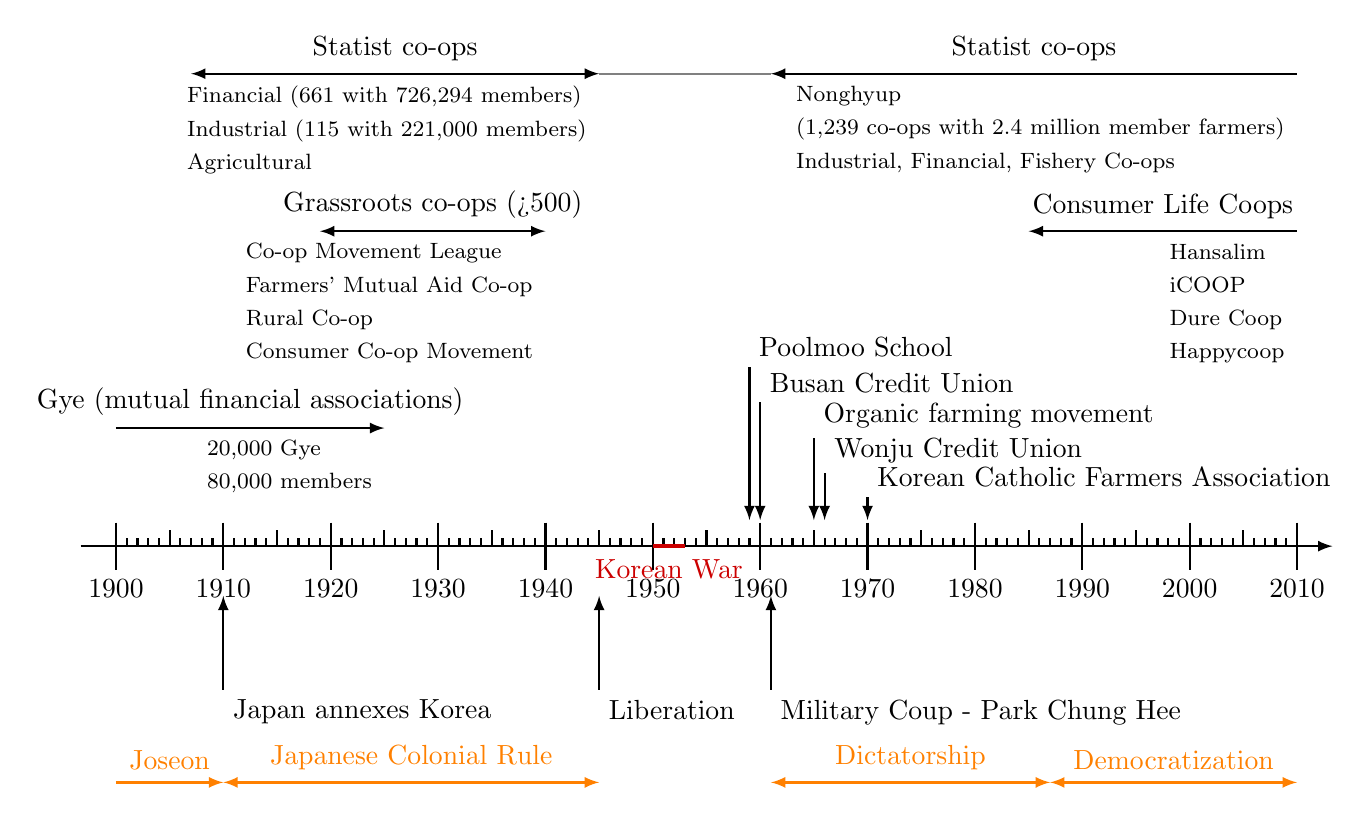
\begin{tikzpicture}[]
  % limits
  \newcount\yearOne; \yearOne=1900
  \def\w{15}    % width of axes
  \def\n{11}     % number of decades
  \def\lt{0.3} %  ten tick length
  \def\lf{0.2} % five tick length
  \def\lo{0.1} %  one tick length
  
  % help functions
  
        % Timeline labels
  \def\yearLabel(#1,#2){\node[above] at ({(#1-\yearOne)*\w/\n/10},\lt) {#2};}
        % Labelled arrows above and below timeline
  \def\yearArrowLabel(#1,#2,#3,#4){
    \def\xy{{(#1-\yearOne)*\w/\n/10}}; \pgfmathparse{int(#2*100)};
    \ifnum \pgfmathresult<0
      \def\yyp{{(\lt*(0.90+#2))}}; \def\yyw{{(\yyp-\lt*#3)}}
      \draw[<-,thick,black,align=center] (\xy,\yyp) -- (\xy,\yyw) node[below right=-0.2,black,align=left] at (\xy,\yyw) {#4};
    \else
      \def\yyp{{(\lt*(0.10+#2)}}; \def\yyw{{(\yyp+\lt*#3)}}
      \draw[<-,thick,black,align=center] (\xy,\yyp) -- (\xy,\yyw) node[above right=-0.2,black,align=left] at (\xy,\yyw) {#4};
    \fi}
    
        % Horizontal labelled arrows below or above timeline
  \def\yearSpan(#1,#2,#3,#4,#5,#6,#7){
      \def\from{{(#1-\yearOne)*\w/\n/10}};
      \def\to{{(#2-\yearOne)*\w/\n/10}};
      \def\height{{#5}};
        \draw[#6,thick,black!20!,color={#7}]
        (\from,\height) -- (\to,\height)
        node[below left=0.8pt,align=left] {#4}
        node[midway,above=0.8pt] {#3};
        }
        
        % Red labelled markers on the timeline itself
    \def\markerLabel(#1,#2,#3,#4){
        \def\from{{(#1-\yearOne)*\w/\n/10}};
        \def\to{{(#2-\yearOne)*\w/\n/10}};
        \def\height{{#4}};
            \draw[-,ultra thick,black!20!red]
            (\from,0) -- (\to,0)
            node[midway,below=#4] {#3};
    }
  
  % axis
  %\draw[thick] (0,0) -- (\w,0);
  \draw[->,thick] (-\w*0.03,0) -- (\w*1.03,0);
  
  % ticks
  \foreach \tick in {0,1,...,\n}{
    \def\x{{\tick*\w/\n}}
    \def\year{\the\numexpr \yearOne+\tick*10 \relax}
  	\draw[thick] (\x,\lt) -- (\x,-\lt) % ten tick
	             node[below] {\year};
	
	\ifnum \tick<\n
	  \draw[thick] ({(\x+\w/\n/2)},0) -- ({(\x+\w/\n/2)},\lf); % five tick
      \foreach \ticko in {1,2,3,4,6,7,8,9}{
        \def\xo{{(\x+\ticko*\w/\n/10)}}
  	    \draw[thick] (\xo,0) -- (\xo,\lo);  % one tick
	}\fi
  }
  
  % MARKERS
    \markerLabel(1950,1953,Korean War,0.8)
  
  % SITUATION
    %STATE CO-OPS
        \yearSpan(1907,1945,Statist co-ops,\footnotesize{Financial (661 with 726,294 members)}\\
        \footnotesize{Industrial (115 with 221,000 members)}\\
        \footnotesize{Agricultural},6,<->,black)
        \yearSpan(1945,1961,,,6,-,gray)
        \yearSpan(1961,2010,Statist co-ops,\footnotesize{Nonghyup}\\
        \footnotesize{(1,239 co-ops with 2.4 million member farmers)}\\
        \footnotesize{Industrial, Financial, Fishery Co-ops},6,<-,black)

    %INDEPENDENT CO-OPS
        \yearSpan(1919,1940,{Grassroots co-ops (>500)},\footnotesize{Co-op Movement League}\\
            \footnotesize{Farmers' Mutual Aid Co-op}\\
            \footnotesize{Rural Co-op}\\
            \footnotesize{Consumer Co-op Movement},4,<->,black)
    %SOCIAL MOVEMENTS & GRASS ROOTS ORGANIZATIONS
        \yearSpan(1900,1925,{Gye (mutual financial associations)},\footnotesize{20,000 Gye}\\
            \footnotesize{80,000 members},1.5,->,black)
    %Consumer Life co-ops
        \yearSpan(1985,2010,{Consumer Life Coops},\footnotesize{Hansalim}\\
            \footnotesize{iCOOP}\\
            \footnotesize{Dure Coop}\\
            \footnotesize{Happycoop}\\
            ,4,<-,black)

  % EVENTS
    \yearArrowLabel(1910,-3,4,Japan annexes Korea)
    \yearArrowLabel(1945,-3.0,4,Liberation)
    \yearArrowLabel(1959,1,6.5,Poolmoo School)
    \yearArrowLabel(1960,1,5,Busan Credit Union)
    \yearArrowLabel(1961,-3,4,Military Coup - Park Chung Hee)
    \yearArrowLabel(1965,1,3.5,Organic farming movement)
    \yearArrowLabel(1966,1,2,Wonju Credit Union)
    \yearArrowLabel(1970,1,1,Korean Catholic Farmers Association)
    %\yearArrowLabel(1961,1.0,1.5,Nonghyup)
    %\yearArrowLabel(1987,1.0,1.5,Hansalim)
    
  %PERIODS
    \yearSpan(1900,1910,Joseon,,-3,->,orange)
    \yearSpan(1910,1945,Japanese Colonial Rule,,-3,<->,orange)
    \yearSpan(1961,1987,Dictatorship,,-3,<->,orange)
    \yearSpan(1987,2010,Democratization,,-3,<->,orange)
  
\end{tikzpicture}

\end{document}


% function written into ~/.zshrc file:
%function tikz2png() {
%    # 1. Check input
%    if [ -z "$1" ]; then
%        echo "Usage: tikz2png path/to/filename.tex"
%        return 1
%    fi
%
%    local input_file="$1"
%    # Get the folder where the .tex file lives
%    local dir_name=$(dirname "$input_file")
%    # Get the filename without extension
%    local base_name=$(basename "$input_file" .tex)
%
%    echo "⚙️  Processing ${base_name} inside ${dir_name}/..."
%
%    # 2. Compile specifically into the target directory
%    # -output-directory ensures the .pdf ends up next to the .tex, not in root
%    pdflatex -output-directory "$dir_name" "$input_file" > /dev/null
%
%    # 3. Check if PDF was created successfully
%    if [ ! -f "${dir_name}/${base_name}.pdf" ]; then
%        echo "❌ Error: PDF creation failed. Check for LaTeX errors."
%        return 1
%    fi
%
%    echo "📸 Converting PDF to PNG..."
%    
%    # 4. Convert using the full path
%    pdftoppm -png -r 300 -singlefile "${dir_name}/${base_name}.pdf" "${dir_name}/${base_name}"
%
%    # 5. Cleanup the specific artifacts in that folder
%    rm "${dir_name}/${base_name}.pdf" "${dir_name}/${base_name}.log" "${dir_name}/${base_name}.aux"
%
%    echo "✅ Success! Saved to ${dir_name}/${base_name}.png"
%}